\section{Extra robustness tests}

\subsection{Scale dependent systematics}\label{sec:scalesys}
Our fiducial cross power spectrum diagnostic (equation \ref{eq:cx_chi2}) uses harmonic modes up to $\ell=20$, which determines the smallest scale used for characterizing residual systematic errors. To investigate the statistical significance of the cross power spectrum's $\chi^{2}$, we examine its dependence on the largest harmonic mode $\ell_{\rm max}$. We extend $\ell_{\rm max}$ from $20$ to $100$, where the latter scale corresponds to density fluctuations on scales smaller than $2$ degrees. Figure \ref{fig:chi2cellextend} shows the median of the cross power spectrum's $\chi^{2}$ from the clean $\fnl=0$ mocks as the highest mode $\ell_{\rm max}$ increases from $20$ to $100$ (represented by the solid line). The red circles and blue crosses show the $\chi^{2}$ values for our sample cleaned respectively with the linear and neural network approaches, both with three maps. Overall, we find that for all scales up to $\ell=100$, the nonlinear three maps approach yields consistent values with the clean mocks, whereas the linear three maps approach exhibits significant remaining systematics at more than 95\% confidence.

\begin{figure}
\centering
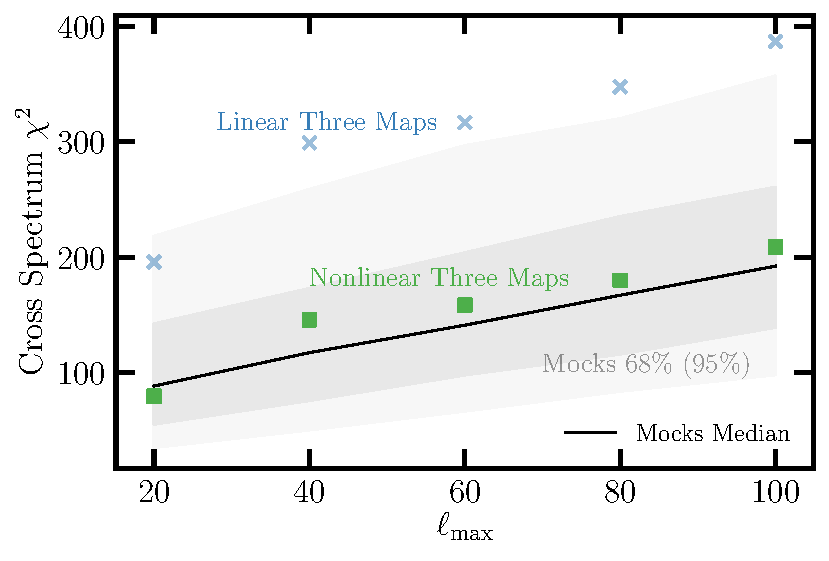
\includegraphics[width=0.45\textwidth]{chi2lmax.pdf}
\caption{The cross power spectrum's $\chi^{2}$ between the LRG density and imaging systematic maps as a function of the highest mode $\ell_{\rm max}$ when the sample is cleaned with the linear (triangles) and non-linear (squares) three maps. The lowest mode is fixed at $\ell_{\rm min}=2$. The solid curve and dark (light) shade represent the median value and $68\%$ ($95\%$) confidence regions, estimated from the $\fnl=0$ mocks.}\label{fig:chi2cellextend}
\end{figure}


\subsection{Redshift uncertainties}\label{ssec:nzuncer}
We use the Early Data Assembly Version 1 (EDA V1) to construct the redshift distribution for the DESI LRG targets. We find that the change in the maximum likelihood estimate of $\fnl$ is negligible, $\Delta \fnl=-1$, \mr{compared to the statistical precision of our measurements}. Figure \ref{fig:cl_nz} shows the measured power spectrum of the DESI targets and the corresponding best fit theory curves. The variations in $dN/dz$ do not significicantly alter the conclusion of our paper.
\begin{figure}
\raggedleft
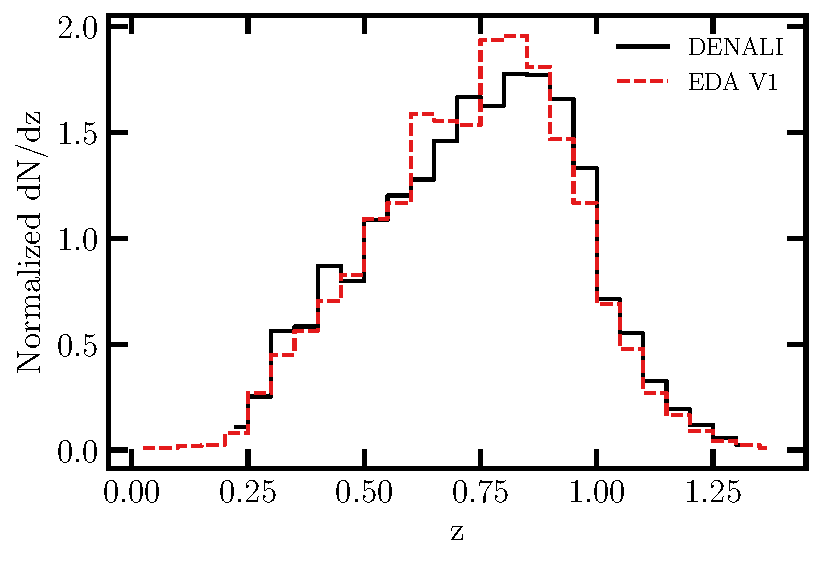
\includegraphics[width=0.42\textwidth]{figures/nz_lrg_eda.pdf}
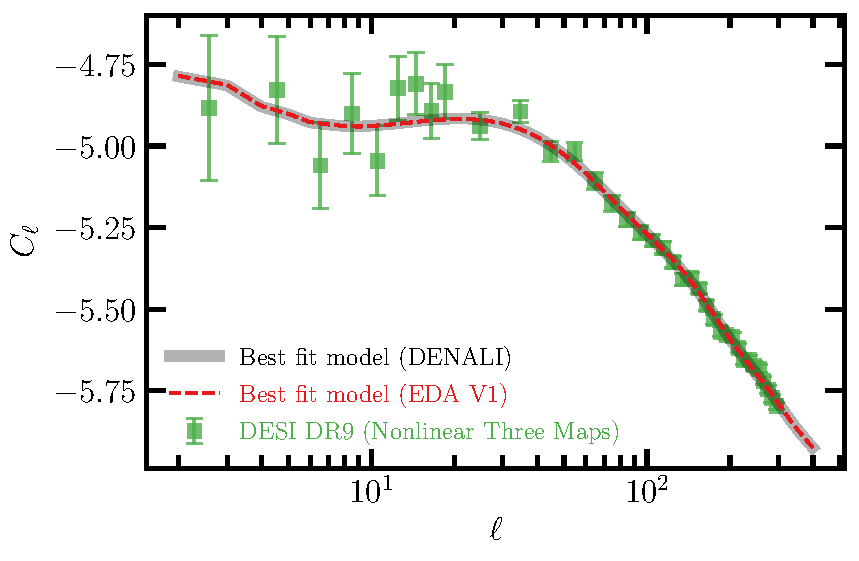
\includegraphics[width=0.45\textwidth]{figures/cl_nz.pdf}\caption{Top: Redshift distribution of the DESI LRG targets from the EDA V1 and Denali. Bottom: The measured power spectrum of the DESI DR9 LRG sample and the best fit theory models using different redshift distributions.}\label{fig:cl_nz}
\end{figure}




\subsection{Spurious bump in NGC}\label{ssec:ndecalsbump}
As shown in Figure \ref{fig:mcmc_dr9elmin} (top panel), we realize that the spurious feature at $\ell \sim 10-20$ is removed in the DECaLS South region after mitigation, but it remains in the BASS+MzLS and DECaLS North. We use the neural networks trained on the DECaLS South with three and nine maps to mitigate the galaxy density in the DECaLS North region, and then measure the power spectrum. Figure \ref{fig:clSonN} shows the power spectrum before treatment (No Weight) and after the nonlinear three maps and nine maps methods for comparison. We find that whatever causing the bump is different between the DECaLS North and South. The best-fit estimates for $\fnl$ from the DR9 DECaLS North using the neural network correction with three maps (NN trained on DECaLS North), three maps (NN trained on DECaLS South), and nine maps (NN trained on DECaLS South) are $41$, \mr{$36$}, and \mr{$75$}, respectively. \mr{The best-fit estimate $\fnl$ from the same data without correction ('No Weight') is 94.}

\begin{figure}
    \centering
    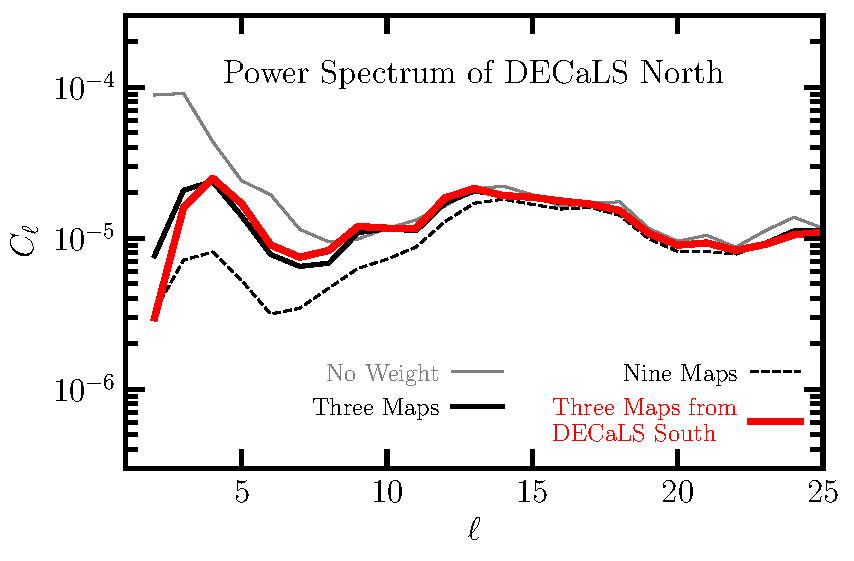
\includegraphics[width=0.45\textwidth]{figures/cl_SonN.pdf}
    \caption{The unbinned measured power spectrum of the DESI LRG targets in the DECaLS North region before and after various mitigations using the neural network approach.}
    \label{fig:clSonN}
\end{figure}


\section{Lognormal mocks}
We fit the mean power spectrum of the lognormal mocks to validate the modeling pipeline, and in particular the survey geometry and integral constraint treatments. We investigate the impact of covariance matrix on the inference of $\fnl$. Finally, we show the impact of imaging systematic mitigation and the over-subtraction effect when the cleaning methods are applied to the mocks. 

\subsection{Clean mocks}
The $68\%$ and $95\%$ probability contours on the PNG parameter $\fnl$ and bias coefficient $b$ are shown in Figure \ref{fig:mcmc_mocks0} and \ref{fig:mcmc_mocks100}, respectively, for the $\fnl=0$ and 76.9 mocks. The best-fitting, marginalized mean estimates, as well as the $1\sigma$ and $2\sigma$ confidence intervals of $\fnl$ are summarized in Table \ref{tab:mocksmcmc}. 


\begin{table*}
  %\begin{center}
    \caption{best-fitting and marginalized mean estimates for $\fnl$ from fitting the mean power spectrum of the mocks. \mr{The covariance is scaled to represent the error on the mean power spectrum.} Degree of freedom is 34 (37 data points - 3 parameters).}   
    \label{tab:mocksmcmc}  
   \centerline{%
    \begin{tabular}{llllllll}
    \hline
    \hline
   &  & & & & $\fnl$ &  \\
   \cmidrule(r{.7cm}){4-7}    
Mock / $\fnl$ &  Footprint   &  Observable & 	Best fit  & Mean & $ 68\%$ CL & $ 95\%$ CL & $\chi^{2}$ \\
    \hline
Clean $76.9$ & DESI & log$C_{\ell}$    & $ 77.67$& $ 77.67$& $ 77.17<\fnl< 78.16$& $ 76.71<\fnl< 78.64$ &   38.8\\
Clean $76.9$ & DESI & $C_{\ell}$       & $ 77.67$& $ 77.65$& $ 77.17<\fnl< 78.14$& $ 76.70<\fnl< 78.60$ &   39.0\\
Clean $76.9$ & DESI & log$C_{\ell}$ + $f_{\rm NL}=0$ cov & $ 77.70$& $ 77.71$& $ 77.25<\fnl< 78.17$& $ 76.81<\fnl< 78.63$ &   39.9\\
Clean $76.9$ & DESI & $C_{\ell}$ + $f_{\rm NL}=0$ cov & $ 77.03$& $ 77.02$& $ 76.93<\fnl< 77.12$& $ 76.83<\fnl< 77.22$ &  207.6\\
\hline
Clean $0$ & DESI         &  log$C_{\ell}$ & $  0.36$& $  0.36$& $  0.06<\fnl<  0.65$& $ -0.23<\fnl<  0.94$ &   35.7\\
Clean $0$ & BASS+MzLS    &  log$C_{\ell}$ & $  0.83$& $  0.82$& $  0.25<\fnl<  1.40$& $ -0.31<\fnl<  1.96$ &   39.4\\
Clean $0$ & DECaLS North &  log$C_{\ell}$& $  0.07$& $  0.06$& $ -0.47<\fnl<  0.60$& $ -1.00<\fnl<  1.12$ &   26.7\\
Clean $0$ & DECaLS South &  log$C_{\ell}$& $  0.67$& $  0.67$& $  0.13<\fnl<  1.22$& $ -0.40<\fnl<  1.75$ &   34.3\\
\hline
    \end{tabular}
    }
\end{table*}


\begin{figure}
    \centering
    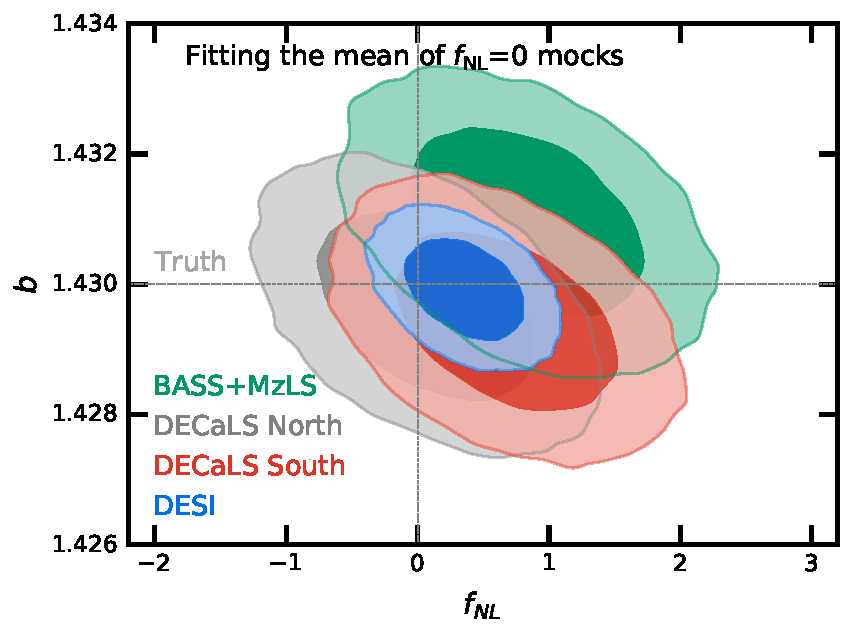
\includegraphics[width=0.45\textwidth]{figures/mcmc_zero.pdf} 
    \caption{68\% and 95\% confidence contours from the mean power spectrum of the $\fnl=0$ mocks for the DESI footprint and sub-imaging surveys. The truth values are represented by vertical and horizontal lines.}\label{fig:mcmc_mocks0}
\end{figure}

\begin{figure}
    \centering
    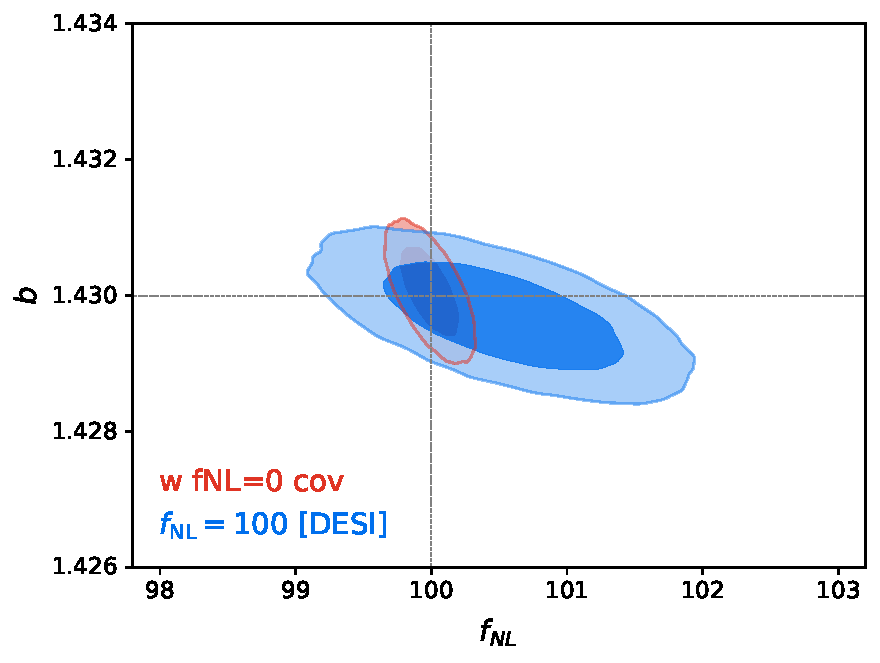
\includegraphics[width=0.45\textwidth]{figures/mcmc_po100.pdf} 
    \caption{68\% and 95\% confidence contours of fitting the mean power spectrum or its log transformation from the $\fnl=76.9$ mocks for the DESI footprint. Using the $\log C_{\ell}$ fitting yield constraints that are insensitive to the covariance used. The truth values are represented by vertical and horizontal lines.}\label{fig:mcmc_mocks100}
\end{figure}

Measuring the power spectrum from the entire DESI footprint reduces the cosmic variance and thus improves the constraining power. Figure \ref{fig:mcmc_mocks0} compares the constraints from fitting the log of the mean power spectrum of the mocks when it is measured from the DESI footprint to those obtained from the sub imaging surveys. We find that the underlying true $\fnl$ value is recovered within $95\%$ confidence, and that the contours for the DESI region are smaller by a factor of two. 

The power spectrum of the mocks at low $\ell$ is very sensitive to the cosmic variance and the true value of $\fnl$. Consequently, a large value of $\fnl$ can induce very large power on low $\ell$, and thus significantly change the covariance matrix. We find that applying the log transformation on the power spectrum makes the result more robust against the choice of the covariance matrix. Figure \ref{fig:mcmc_mocks100} shows the confidence contours when we fit either the power spectrum or its log transform of the $\fnl=76.9$ mocks, and use different covariance matrices. We consider the $\fnl=0$ and $76.9$ mocks to construct the covariance from one set and use it to fit the mean power spectrum of the other set. When the covariance matrix is constructed from the same set of mocks used for the mean power spectrum, we find that the difference in $\fnl$ constraints between fitting the power spectrum and its log transformation is negligible at only 2\%. If we use the $\fnl=0$ mocks to estimate the covariance, and fit the log power spectrum of the $\fnl=76.9$ mocks, we find that the error on $\fnl$ increases only by $7\%$. However, when the mean power spectrum of the $\fnl=76.9$ mocks is fit using the covariance matrix estimated from the $\fnl=0$ mocks, the constraints tighten by a factor of $5$ due to a higher signal to noise ratio. Therefore, we argue that fitting the log power spectrum can help mitigate the need for having $\fnl$-dependent covariance matrices and make the constraints less sensitive to covariance construction.

\begin{figure}
    \centering    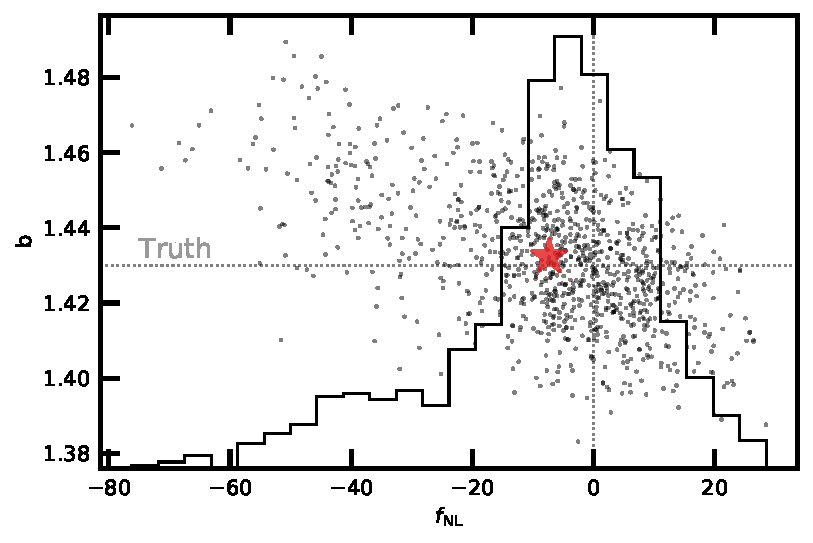
\includegraphics[width=0.45\textwidth]{figures/bestfit_zero.pdf} 
    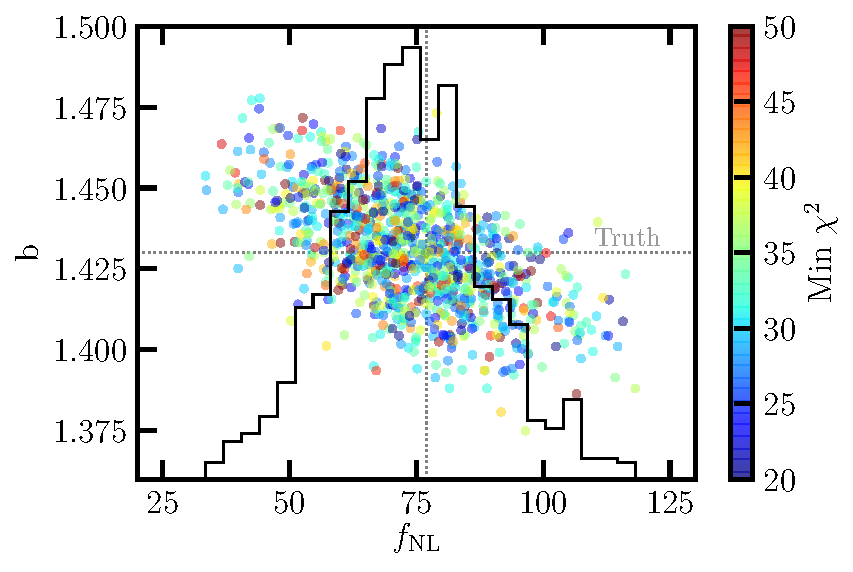
\includegraphics[width=0.45\textwidth]{figures/bestfit_po100.pdf}         
    \caption{best-fitting estimates from fitting 1000 lognormal mocks with $\fnl=0$ (top) and $76.9$ (bottom) in the DESI footprint. The truth values are represented by vertical and horizontal lines. The truth values are represented by vertical and horizontal lines.}\label{fig:bestfit_mocks}
\end{figure}


Figure \ref{fig:bestfit_mocks} shows the best-fitting estimates for $b$ vs $\fnl$ for $\fnl=0$ and $=76.9$ mocks in the top and bottom panels, respectively. Truth values are represented via the dotted lines. The points are color-coded with the minimum $\chi^{2}$ from fit for each realization. The histograms of best-fitting $\fnl$ estimates are plotted in the background. For the $\fnl=0$ mocks, the best-fitting estimates are more symmetric. To understand this behaviour, we consider the first derivative of the likelihood (Equation \ref{eq:likelihood}), which is proportional to the first derivative of the log power spectrum. By simplifying the integrals involved in $C_{\ell}$, we have $C_{\ell} = A_{0, \ell} + A_{1,\ell} \fnl + A_{2, \ell} \fnl^{2}$ where $A_{123,\ell}$ are $\ell$-dependent terms. Then, the derivative of the likelihood is equivalent to
\begin{equation}
    \frac{d}{d\fnl}\log(C_{\ell}) = \frac{A_{1, \ell}+2A_{2, \ell}\fnl}{A_{0, \ell} + A_{1,\ell} \fnl + A_{2, \ell} \fnl^{2}}.
\end{equation}
For infinitesimal values of $\fnl$, the derivative becomes asymptotically independent from $\fnl$ while for large values of $\fnl$ is decreases as $2/\fnl$. This implies that for the $\fnl=0$ mocks, the likelihood is more likely to be skewed toward negative values.

\subsection{Contaminated mocks}
Our nonlinear neural network-based approach is applied to the $\fnl=0$ and $76.9$ mocks. We only consider the methods that include running the neural network with three, four, and nine imaging systematic maps. The measured mean power spectrum of the mocks are shown in Figure \ref{fig:clmocks} for $\fnl=0$ (left) and $76.9$ (right). The solid and dashed curves show the measurements respectively from the clean and contaminated mocks.

\begin{figure*}
    \centering
    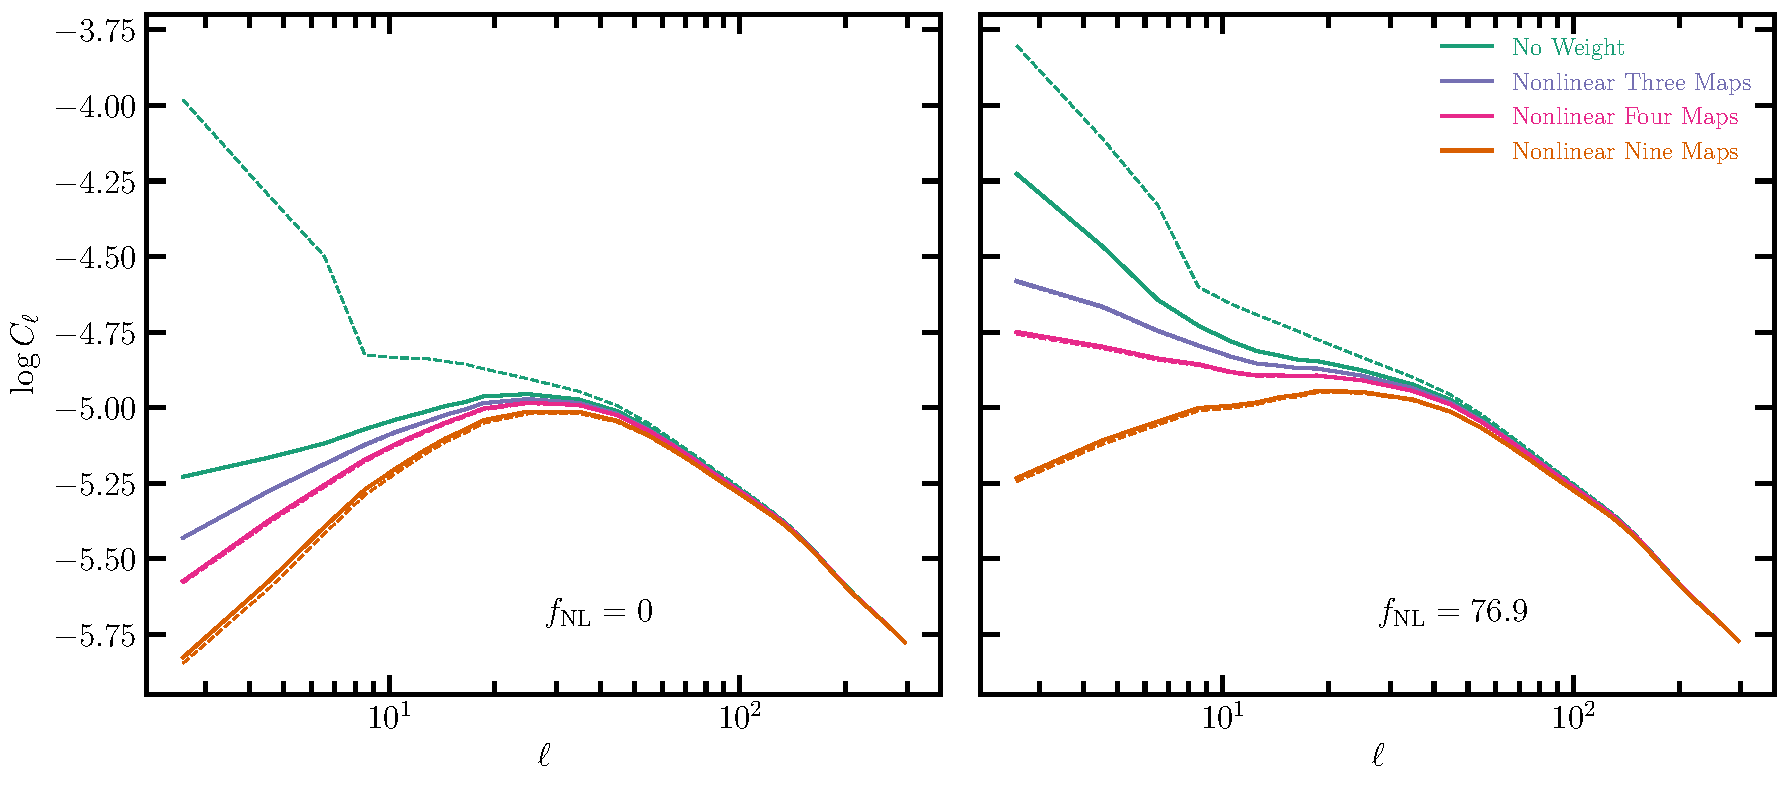
\includegraphics[width=0.9\textwidth]{figures/clmocks.pdf}
    \caption{The mean power spectrum of the $\fnl =0$ and $76.9$ mocks with (dashed) and without (solid) imaging systematics before ('No Weight') and after applying the non-linear cleaning method with three, four, and nine maps.}\label{fig:clmocks}
\end{figure*}


We find that the imaging treatment has removed some of the true clustering signal, and the amount of the over-subtraction is almost the same regardless of whether the mocks have systematics. The over-subtraction induces biases in the $\fnl$ constraints, as summarized in Table \ref{tab:contmocksmcmc}. The over-subtraction at low $\ell$ is so high that we get a poor fit after applying the mitigation with the nonlinear three maps approach, e.g., $\chi^{2}=86.8$ for the clean $\fnl=0$ mocks.


\begin{table*}
  %\begin{center}
    \caption{best-fitting and marginalized estimates for $\fnl$ from fitting the mean power spectrum of the mocks before and after corrections using the non-linear approach with various combinations of the imaging systematic maps. \mr{The covariance is scaled to represent the error on the mean power spectrum.} The estimates are not accounted for over-correction, and therefore are subject to mitigation systematics.}   
    \label{tab:contmocksmcmc}  
   \centerline{%
    \begin{tabular}{lllllll}
    \hline
    \hline
   &  & 	   & & $\fnl$ + Mitigation Systematics & & \\
   \cmidrule(r{.7cm}){3-6}    
Mock / $\fnl$ & Method & Best fit  & Mean & $ 68\%$ CL & $ 95\%$ CL & $\chi^{2}$ \\
    \hline
Clean $0$ & No Weight                   & $  0.36$& $  0.36$& $  0.06<\fnl<  0.65$& $ -0.23<\fnl<  0.94$ &   35.7\\
Clean $0$ & Three Maps                  & $-11.64$& $-11.65$& $-12.00<\fnl<-11.30$& $-12.34<\fnl<-10.97$ &   86.8\\
Clean $0$ & Four Maps                   & $-20.14$& $-20.13$& $-20.44<\fnl<-19.82$& $-20.74<\fnl<-19.52$ &  472.8\\
Clean $0$ & Nine Maps                   & $-26.91$& $-26.92$& $-27.16<\fnl<-26.68$& $-27.39<\fnl<-26.46$ & 5481.0\\
Contaminated $0$ & Three Maps           & $-12.12$& $-12.13$& $-12.48<\fnl<-11.78$& $-12.83<\fnl<-11.44$ &   94.0\\
Contaminated $0$ & Four Maps            & $-20.97$& $-20.98$& $-21.28<\fnl<-20.67$& $-21.58<\fnl<-20.37$ &  556.3\\
Contaminated $0$ & Nine Maps            & $-28.13$& $-28.13$& $-28.36<\fnl<-27.90$& $-28.59<\fnl<-27.67$ & 6760.5\\
\hline
Clean $76.9$ & No Weight               & $ 77.67$& $ 77.67$& $ 77.17<\fnl< 78.16$& $ 76.71<\fnl< 78.64$ &   38.8\\
Clean $76.9$ & Three Maps              & $ 54.57$& $ 54.57$& $ 54.14<\fnl< 55.01$& $ 53.72<\fnl< 55.45$ &  603.5\\
Clean $76.9$ & Four Maps               & $ 38.38$& $ 38.38$& $ 37.99<\fnl< 38.78$& $ 37.60<\fnl< 39.16$ &  537.0\\
Clean $76.9$ & Nine Maps               & $  6.04$& $  6.04$& $  5.72<\fnl<  6.36$& $  5.41<\fnl<  6.67$ &  694.0\\
Contaminated $76.9$ & Three Maps       & $ 54.01$& $ 54.00$& $ 53.57<\fnl< 54.44$& $ 53.15<\fnl< 54.86$ &  588.0\\
Contaminated $76.9$ & Four Maps        & $ 37.48$& $ 37.49$& $ 37.09<\fnl< 37.88$& $ 36.70<\fnl< 38.27$ &  510.7\\
Contaminated $76.9$ & Nine Maps        & $  4.59$& $  4.58$& $  4.26<\fnl<  4.90$& $  3.95<\fnl<  5.22$ &  649.7\\
\hline
    \end{tabular}
    }
\end{table*}
Using the calibration parameters presented in \S \ref{ssec:calibration}, we account for the shift in the $\fnl$ constraints caused by the imaging systematic mitigation. We show the marginalized probability distributions on $\fnl$ before and after accounting for the over-correction in the right and left panels of Figure \ref{fig:contmcmc}.

\begin{figure*}
\centering
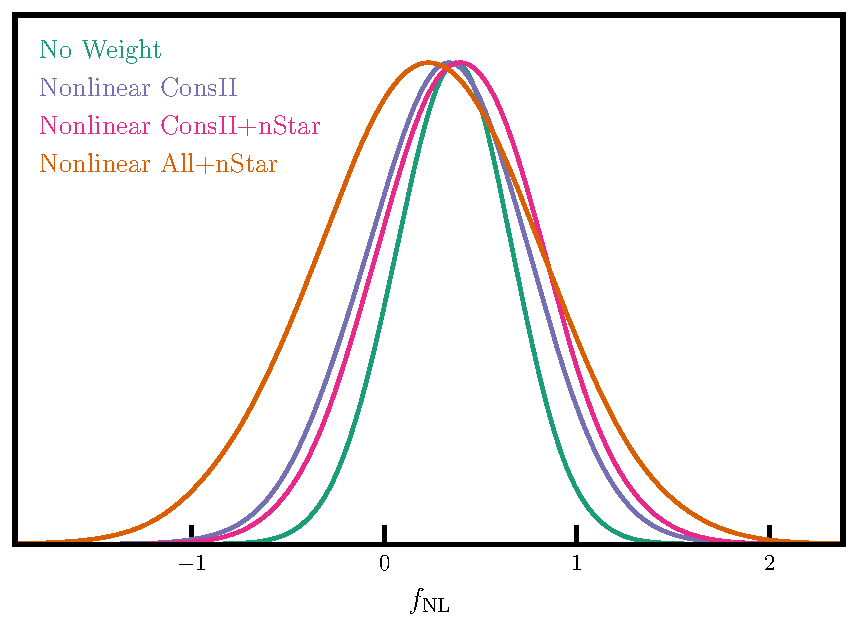
\includegraphics[width=0.45\textwidth]{figures/mcmc_cont.pdf}
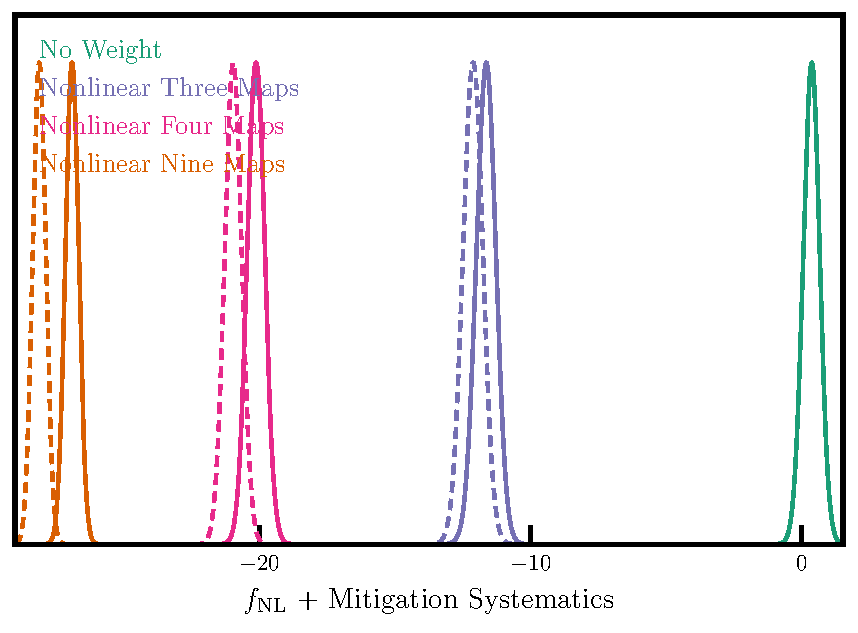
\includegraphics[width=0.45\textwidth]{figures/mcmc_contnoshift.pdf}
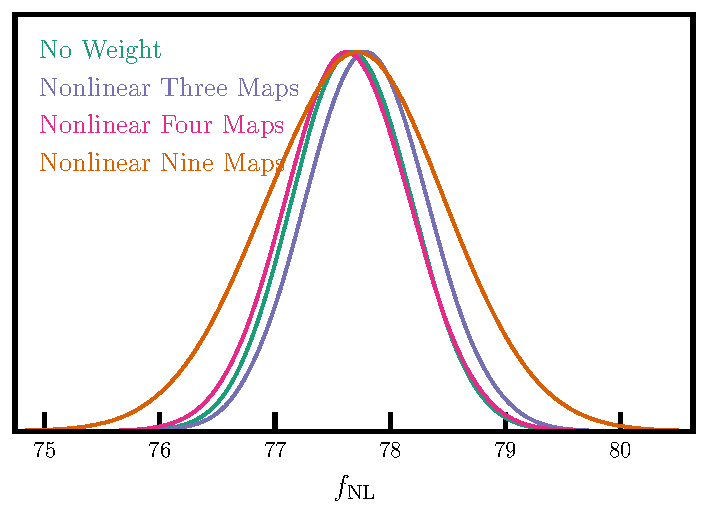
\includegraphics[width=0.45\textwidth]{figures/mcmcp_cont.pdf}
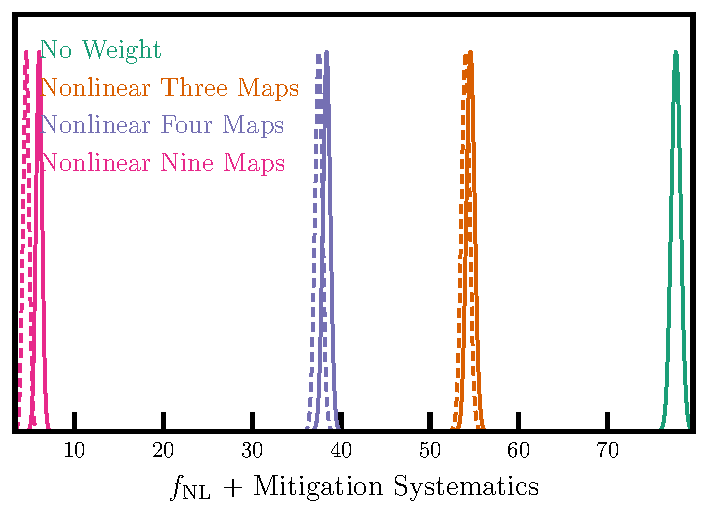
\includegraphics[width=0.45\textwidth]{figures/mcmcp_contnoshift.pdf}
\caption{Probability distributions of $\fnl$ from the mean power spectrum of the $\fnl=0$ (top) and $\fnl=76.9$ (bottom) mocks before and after mitigation with the non-linear methods using three, four, and nine maps. The dashed (solid) curves show the distributions for the contaminated (clean) mocks. Left: The posteriors are adjusted to account for the over-correction effect. Right: The posteriors are subject to the over-correction effect, and thus the scaling of $\fnl$ values is biased due to mitigation.}\label{fig:contmcmc}
\end{figure*}


% \section{Redshift distribution}
% Redshift distribution of LRGs is constructed from the DESI SV data release of Denali with the same selection. The fiducial distribution only covers the redshift range from 0.2 to 1.35. Below we test the impact of LRG dN/dz on the angular power spectrum.


% \begin{figure}
% \centering
% 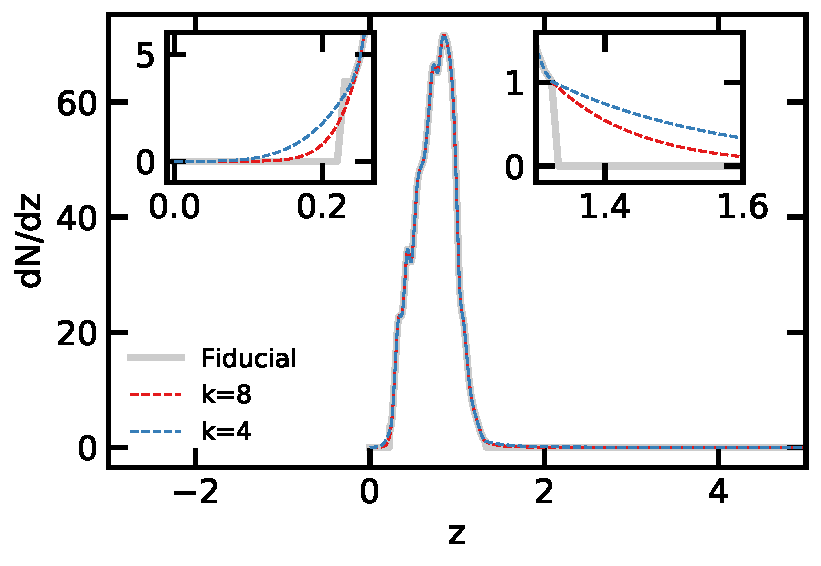
\includegraphics[width=0.45\textwidth]{nztreat.pdf}
% 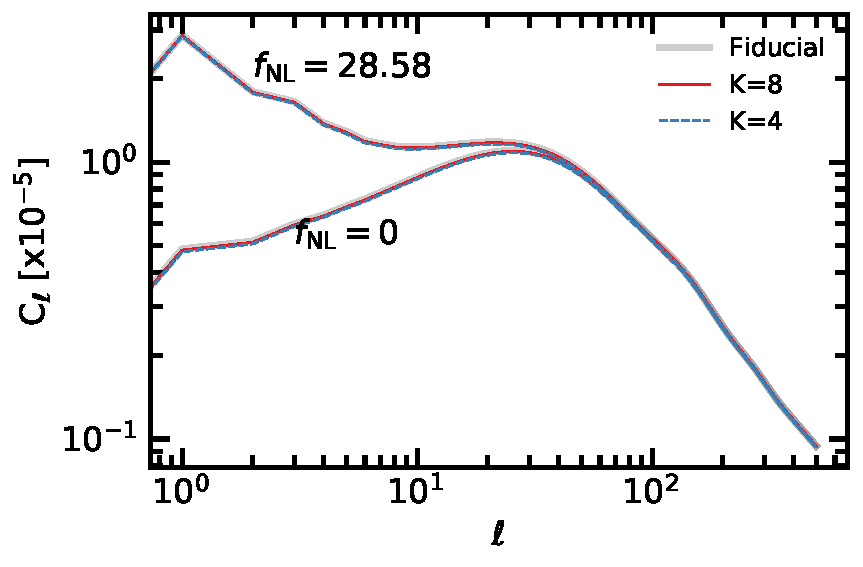
\includegraphics[width=0.45\textwidth]{cell_nz.pdf}
% \caption{Top: Redshift distribution of LRGs. Bottom: Power spectrum given various dN/dz treatments for two arbitrary $\fnl$ values.}
% \end{figure}